\documentclass[10pt]{article}
\usepackage[margin=1in, paperwidth=8.5in, paperheight=11in]{geometry}
\usepackage{ifpdf,amsmath, amssymb, comment, color, graphicx, stmaryrd,setspace,enumitem,tikz, fancyhdr, wrapfig, textcomp, mathptmx, siunitx, pdfpages}
\usepackage[colorlinks]{hyperref}
\usepackage{tikz}
\usetikzlibrary{trees}

\setlength{\headheight}{14.5pt}
\newcommand{\Q}{\mathbb{Q}}
\newcommand{\R}{\mathbb{R}}
\newcommand{\Z}{\mathbb{Z}}
\newcommand{\vu}{\mathbf{u}}
\newcommand{\vv}{\mathbf{v}}
\newcommand{\vw}{\mathbf{w}}
\newcommand{\vi}{\mathbf{i}}
\newcommand{\vj}{\mathbf{j}}
\newcommand{\vk}{\mathbf{k}}
\newcommand{\vn}{\mathbf{n}}
\newcommand{\vr}{\mathbf{r}}
\newcommand{\va}{\mathbf{a}}
\newcommand{\vF}{\mathbf{F}}
\newcommand{\vL}{\mathbf{L}}
\newcommand{\vT}{\mathbf{T}}
\newcommand{\vN}{\mathbf{N}}
\newcommand{\proj}{\operatorname{proj}}
\newcommand{\orth}{\operatorname{orth}}
\newcommand\del\nabla
\newcommand\dotp[1][.5]{\,\mathbin{\vcenter{\hbox{\scalebox{#1}{$\bullet$}}}}\,}

% Solution text is in red. If you want the solutions to show, remove the \iffalse from the definition of the \red command.
%\newcommand{\red}[1]{ %\iffalse
%	\textcolor{red}{#1} }%\fi}

\newenvironment{red}{\color{red}}{\ignorespacesafterend}
\newcommand{\blue}[1]{\textcolor{blue}{#1}}
\newcommand{\green}[1]{\textcolor{green}{#1}}
\renewcommand{\section}[1]{\begin{center} \textbf{#1} \\\end{center}}
%
\hyphenpenalty=5000
\setlength{\parindent}{0in}
%\oddsidemargin=-.25in
\allowdisplaybreaks
\pagestyle{fancy}
\renewcommand{\headrulewidth}{0pt}
\lhead{MATH 203}
\rhead{Fall 2019}
%\lfoot{\copyright\ CLEAR Calculus 2010}
\cfoot{}

\begin{document}
%


%\onehalfspacing
\allowdisplaybreaks
%##################################################################
\section{PS\#11 -- Surface area; triple integrals - \red{Answer key} }

\begin{enumerate}[leftmargin=0pt]
    
    \item WW 3.6 \#2 has you parameterize a cone. Find the surface area of that cone using the formula we developed in class. 
    \textbf{Please feel free to use Wolfram$|$Alpha to compute $\left|\mathbf{r}_s \times \mathbf{r}_t\right|$}. According to the google, your answer should be:
    \[A = \pi r \left(r+\sqrt{h^2+r^2}\right).\]
    
    \begin{red}
    Okay, so everybody's numbers on WW 3.6 \#2 are a little different, so let's solve the problem in general. Let's say we have a cone with height $h$ and base radius $r$. Let's start by parameterizing $x(s, t)$ and $y(s, t)$ to be a circle of radius $s$:
    \begin{align*}
        x(s, t) &= s\cos(t) \\
        y(s, t) &= s\sin(t)
    \end{align*}
    Cool, and now we just have to do something fancy with $z$ such that the radius works out right. Let's see, we want $z=h$ to be where $s=0$, and we want $z=0$ to be where $s=r$. So $z$ is going to depend on $s$ (and $s$ only; $z$ shouldn't depend on the angle $t$ at all) in this kind of way:
    \begin{center}
        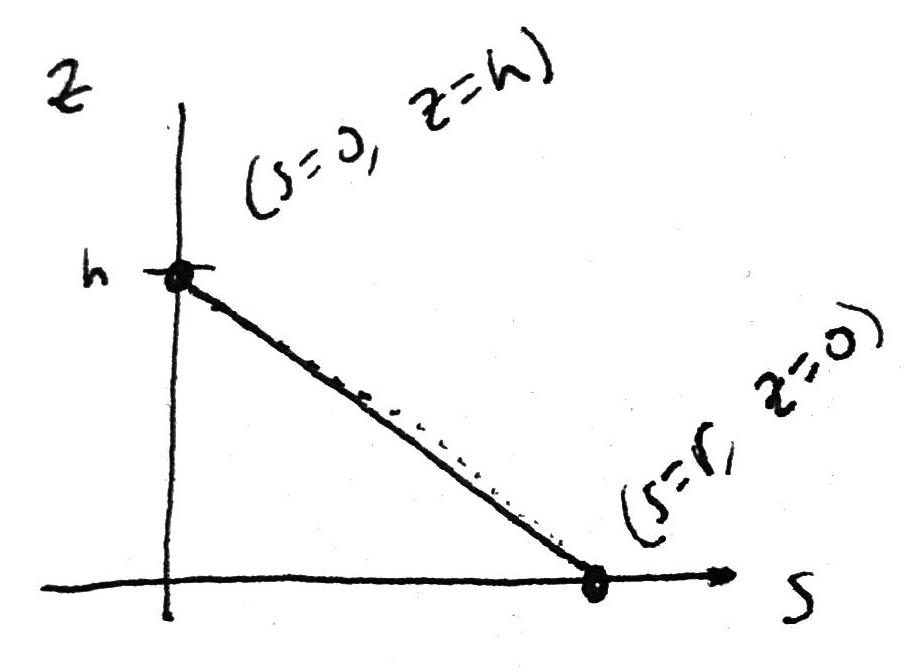
\includegraphics[width=0.3\textwidth]{ps11-z-s.jpg}
    \end{center}
    The slope of this line is $\frac{-h}{r}$ and the intercept is $h$, so:
    \[z(s,t) = \frac{-h}{r}s+h\]
    Therefore, here's our $\mathbf{r}(s,t)$, and its derivatives:
    \begin{align*}
    \mathbf{r}(s,t) &= \left\langle s\cos(t), s\sin(t), \frac{-h}{r}s+h\right\rangle, \quad 0 \leq t \leq 2\pi, \quad 0 \leq s \leq r \\
    \mathbf{r}_s &= \left\langle\cos(t), \sin(t), \frac{-h}{r} \right\rangle \\
    \mathbf{r}_t &= \left\langle -s\sin(t), s\cos(t), 0\right\rangle
    \end{align*}
    Computing $\mathbf{r}_s \times \mathbf{r}_t$ is a good job for Wolfram$|$Alpha, which tells me: 
    \begin{align*}
        \mathbf{r}_s\times\mathbf{r}_t &= 
        \left\langle
        \frac{h s \cos(t)}{r}, \frac{h s \sin(t)}{r}, s \cos^2(t) + s \sin^2(t)\right\rangle = \left\langle
        \frac{h}{r}s \cos(t), \frac{h}{r}s \sin(t), s\right\rangle
        \intertext{(I had to turn on my human brain to simplify this a little, because W$|$A said something unnecessarily complicated.)}
        \left|\mathbf{r}_s \times \mathbf{r}_t\right| &= \sqrt{\frac{h^2}{r^2} s^2 \cos^2(t) + \frac{h^2}{r^2} s^2 \sin^2(t) + s^2}
        = \sqrt{\frac{h^2}{r^2} s^2 +s^2} = s\sqrt{\frac{h^2}{r^2} + 1}
    \end{align*}
    (Again, asking W$|$A what the magnitude of that vector above is yields something unnecessarily complicated. This is a good lesson in the limits of computing technology. W$|$A is programmed to be as general as possible when thinking about what kinds of inputs you're giving it. They might be positive or negative, real or complex, etc. etc., so sometimes it's up to us to turn on our human brains and be like, okay, contextually, all that stuff is positive numbers, so we don't need all these absolute value signs, etc. etc.)
    
    Now we can finally compute the surface area:
    \begin{align*}
        SA &= \iint_D \left|\mathbf{r}_s \times \mathbf{r}_t\right| \, dA \\
        &= \int_{s=0}^r \int_{t=0}^{2\pi} s\sqrt{\frac{h^2}{r^2} + 1}\,dt\,ds 
        = \left(\sqrt{\frac{h^2}{r^2} + 1}\right)\int_{s=0}^r \int_{t=0}^{2\pi} s\,dt\,ds
        \intertext{(That whole square root thing is just a constant, as far as $s$ and $t$ are concerned.)}
        &= \left(\sqrt{\frac{h^2}{r^2} + 1}\right) \int_{s=0}^r\left[st\right|_{t=0}^{2\pi}\,ds 
        =\left(\sqrt{\frac{h^2}{r^2} + 1}\right) \int_{s=0}^r 2\pi s\,ds \\
        &= \left(\sqrt{\frac{h^2}{r^2} + 1}\right) \left[ 2\pi\frac{s^2}{2}\right|_{s=0}^r = \left(\sqrt{\frac{h^2}{r^2} + 1}\right) \cdot \pi r^2
        = \pi r^2\sqrt{\frac{h^2+r^2}{r^2}} = \pi r \sqrt{h^2+r^2}.
    \end{align*}
    Hmm, that looks pretty close to what google said, but google also had this extra $\pi r^2$. Oh, wait, that makes sense, that's the area of the \textbf{bottom} of the cone, and this integral only tells us the area of the \textbf{sides}. Yay, thanks, human brain!
    \end{red}
\end{enumerate}

\begin{red}
\textbf{Learning Targets Reflection:} HBTs, V1, V2, S3, D6/9, I3, I4, I5 
\end{red}

\end{document}